% !TEX root = ../PolycopiePremiere2627.tex
%%%%%%%%%%%%%%%%%%%%%%%%%%%%%%%%%%%%%%%%%%%%%%%%%%%%%%%%%%%%%%%%%%%%%%%%%%%%%%%%
% Contenu initial repris de Louis Paternault --- http://ababsurdo.fr
%
% Publié sous licence Creative Commons Attribution-ShareAlike 4.0 International (CC BY-SA 4.0)
% http://creativecommons.org/licenses/by-sa/4.0/deed.fr
%%%%%%%%%%%%%%%%%%%%%%%%%%%%%%%%%%%%%%%%%%%%%%%%%%%%%%%%%%%%%%%%%%%%%%%%%%%%%%%%

\chapter{Fonction exponentielle}

\noindent\textbf{Activité}

En un an, le nombre d'abonnés d'une chaîne de vidéos sur un réseau social a augmenté de 30\%. Quel a été le taux d'évolution moyen par mois tout au long de cette année ?

\section{Fonction exponentielle}

\Dfn{On appelle \emph{fonction exponentielle} de base $a$ (où $a$ est un nombre réel strictement positif) la fonction $f$ définie sur $\R$ par $f:x\mapsto a^x$.}

\Prp[Règles de calcul]{Pour tous nombres réels $a$ et $b$ strictement positifs, et tous nombres $x$ et $y$ réels, on a :
\begin{multicols}{2}
\begin{enumerate}[label=(\roman*)]
    \item $a^0=1$
    \item $a^x\times a^y=a^{x+y}$
    \item $\left( a^x \right)^y=a^{x\times y}$
    \item $a^x\times a^{-x}=1$
    \item $a^{-x}=\dfrac{1}{a^x}$
    \item $a^{x-y}=\dfrac{a^x}{a^y}$
    \item $\left(a \times b\right)^x=a^x\times b^x$
\end{enumerate}
\end{multicols}}

\Exemple{Simplifier autant que possible les expressions suivantes :
\begin{enumerate}
    \item $3^{2,5}\times3^{-2}=$
    \item $\dfrac{5^{7}}{5^{2}}=$
    \item $\dfrac{2^{2,5}\times2^{3,5}+\left(2^{1,5}\right)^4}{7,6^0\times2^{4}}=$
\end{enumerate}}

\Prp[Sens de variations]{Soient $k$ et $a$ deux nombres strictement positifs, et $f$ la fonction définie sur $\R$ par $f(x)=k\times a^x$. Alors :
\begin{itemize}
    \item si $0<a<1$, alors la fonction $f$ est strictement décroissante sur $\R$ ;
    \item si $a=1$, alors la fonction $f$ est constante sur $\R$ ;
    \item si $a>1$, alors la fonction $f$ est strictement croissante sur $\R$.
\end{itemize}}

\Exemple{Dresser le tableau de variations de la fonction $f$ définie par $f(x)=4\times\pi^x$.}

\Prp[Courbe représentative]{
\begin{center}
    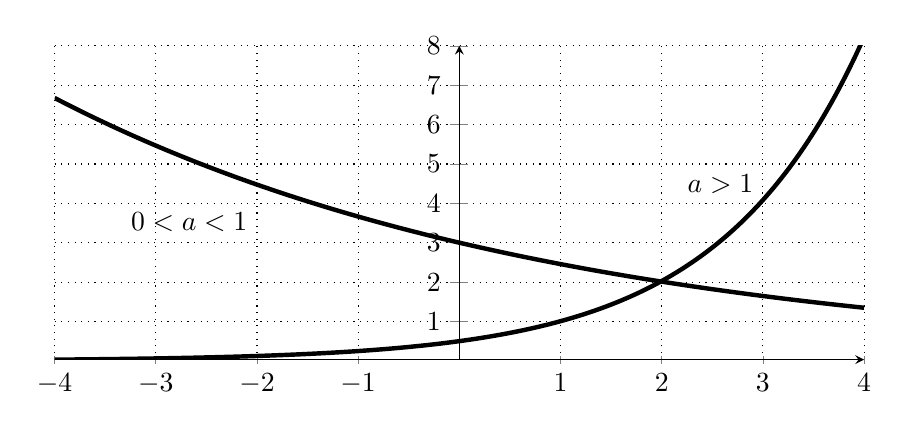
\begin{tikzpicture}
        \begin{axis}[
                xscale=1.5,
                yscale=.7,
                domain=-4:4,
                axis lines=middle,
                xtick={-4, -3, ..., 4},
                ytick={1, 2, ..., 8},
                ymax=8,
                clip=true,
                grid style={dotted,black},
                grid=both,
            ]
            \addplot[black, ultra thick, samples=100,smooth]{.5*exp(.7*x)};
            \addplot[black, ultra thick, samples=100,smooth]{3*exp(-.2*x)};
            \draw (axis cs:-2, 4) node[below left]{$0<a<1$};
            \draw (axis cs:3, 4) node[above left]{$a>1$};
        \end{axis}
    \end{tikzpicture}
\end{center}}

\Exemple{Associer chacune des fonctions suivantes à sa courbe.
\[\begin{array}{*{4}{c}}
    f(x)=3^x&
    g(x)=2\times\left(^1/_3\right)^x&
    h(x)=3\times2^x&
    k(x)=3\times0,5^x\\
\end{array}\]

\begin{center}
    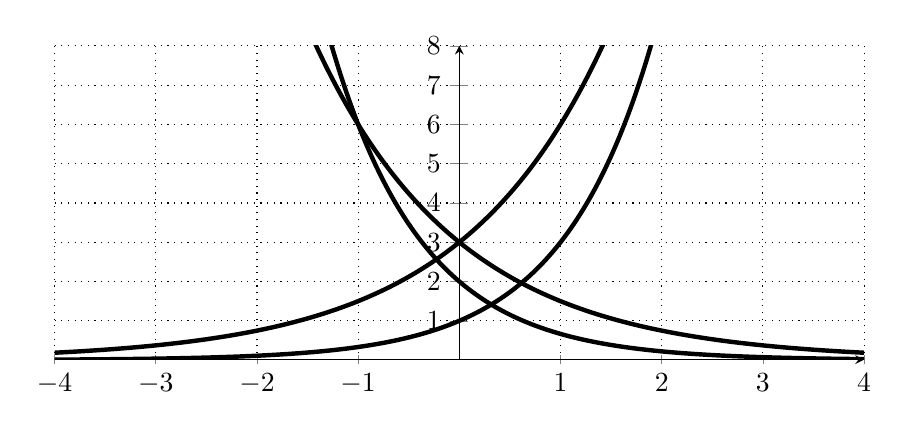
\begin{tikzpicture}
        \begin{axis}[
                xscale=1.5,
                yscale=.7,
                domain=-4:4,
                axis lines=middle,
                xtick={-4, -3, ..., 4},
                ytick={1, 2, ..., 8},
                ymax=8,
                clip=true,
                grid style={dotted,black},
                grid=both,
            ]
            \addplot[black, ultra thick, samples=100,smooth]{1*3^x};
            \addplot[black, ultra thick, samples=100,smooth]{2*.33333^x};
            \addplot[black, ultra thick, samples=100,smooth]{3*2^x};
            \addplot[black, ultra thick, samples=100,smooth]{3*0.5^x};
        \end{axis}
    \end{tikzpicture}
\end{center}}

\section{Racine $n$-ième}

\Prp{Pour tout nombre $a$ positif, l'équation $x^n=a$ admet une unique solution réelle positive : $x=a^{^1/_n}$.}

\Exemple{Résoudre les deux équations suivantes (arrondir au centième).
\begin{enumerate}
    \item $x^4=8$
    \item $4x^7=5x$
\end{enumerate}}

\Exemple{Une biologiste a laissé des bactéries se reproduire pendant exactement 24 heures, et elle a observé que le nombre de ces bactéries a été multiplié par 4. Quel a été le taux d'évolution moyen du nombre de ces bactéries, par heure ?}
